\chapter{基于 IQL 的拥塞控制模型训练与部署实现}
\label{chap:train_iql_model}

\section{离线强化学习范式与 IQL 算法选择}

将强化学习引入 WebRTC 拥塞控制，首先需要解决训练范式的选择问题。在线强化学习要求智能体在训练过程中持续与环境交互，但实时视频通话对服务质量稳定性要求严苛，在线探索过程中的策略崩溃将直接损害用户体验；同时，网络状态空间规模庞大，从零开始的在线学习需要海量交互样本，且其随机探索行为会与现有 GCC 机制产生不可预测的耦合，使训练信号信噪比严重恶化。

上述障碍促使本研究转向离线强化学习。该范式的核心特征是：策略训练完全依赖预先收集的静态数据集，学习过程中不再与环境交互。这一特征天然契合本研究的场景——第\ref{chap:dataset_construction}章已构建了规模化的网络状态-动作-奖励轨迹数据集，其中隐含了 GCC 在多种网络条件下的决策逻辑与效果反馈。离线学习可以从这些数据中提取价值，而无须承担在线探索的风险。

然而，离线学习面临\textbf{分布偏移}（Distributional Shift）这一核心挑战：当学得策略在测试时访问数据集中未充分覆盖的状态-动作对时，价值函数估计可能产生严重偏差。本研究采用的隐式 Q 学习（Implicit Q-Learning, IQL）算法正是为应对该问题设计的解决方案——它通过期望回归机制仅从数据集中已出现动作的上界提取策略，避免了对分布外动作的价值评估，从而在不牺牲稳定性的前提下实现策略改进。

\section{策略与价值网络的架构设计}

IQL 算法需要三类网络协同工作：策略网络 $\pi$、Q 函数 $Q(s,a)$ 与价值函数 $V(s)$。其中策略网络是部署阶段实际运行的对象，其架构设计需充分契合拥塞控制任务的特性。

拥塞控制任务的状态空间具有显著时序依赖：当前时刻的孤立度量值（如 RTT=50ms）无法区分“延迟正在恶化”与“延迟正在恢复”两种截然不同的演化方向，必须结合历史趋势进行综合判断。本研究因此采用基于门控循环单元（GRU）的时序编码器，整体策略网络结构如图\ref{fig:gaussian-policy-arch} 所示：50 维 feature-major 状态向量经线性层映射至 256 维隐空间，再由双层 GRU 对历史窗口进行序列建模以提取长程依赖；GRU 输出经两个残差块进一步提炼高阶特征后，由 Tanh 输出层映射至 $[-1, 1]$ 区间，最终乘以最大动作值（约 12 Mbps）得到带宽估计。残差结构在此扮演了双重角色：缓解深层网络的梯度问题，同时为策略提供“模仿 GCC 基准行为”的捷径——当残差分支输出趋零时，策略退化为对隐状态的恒等映射，对应一种保守决策。

\begin{figure}[htbp]
    \centering
    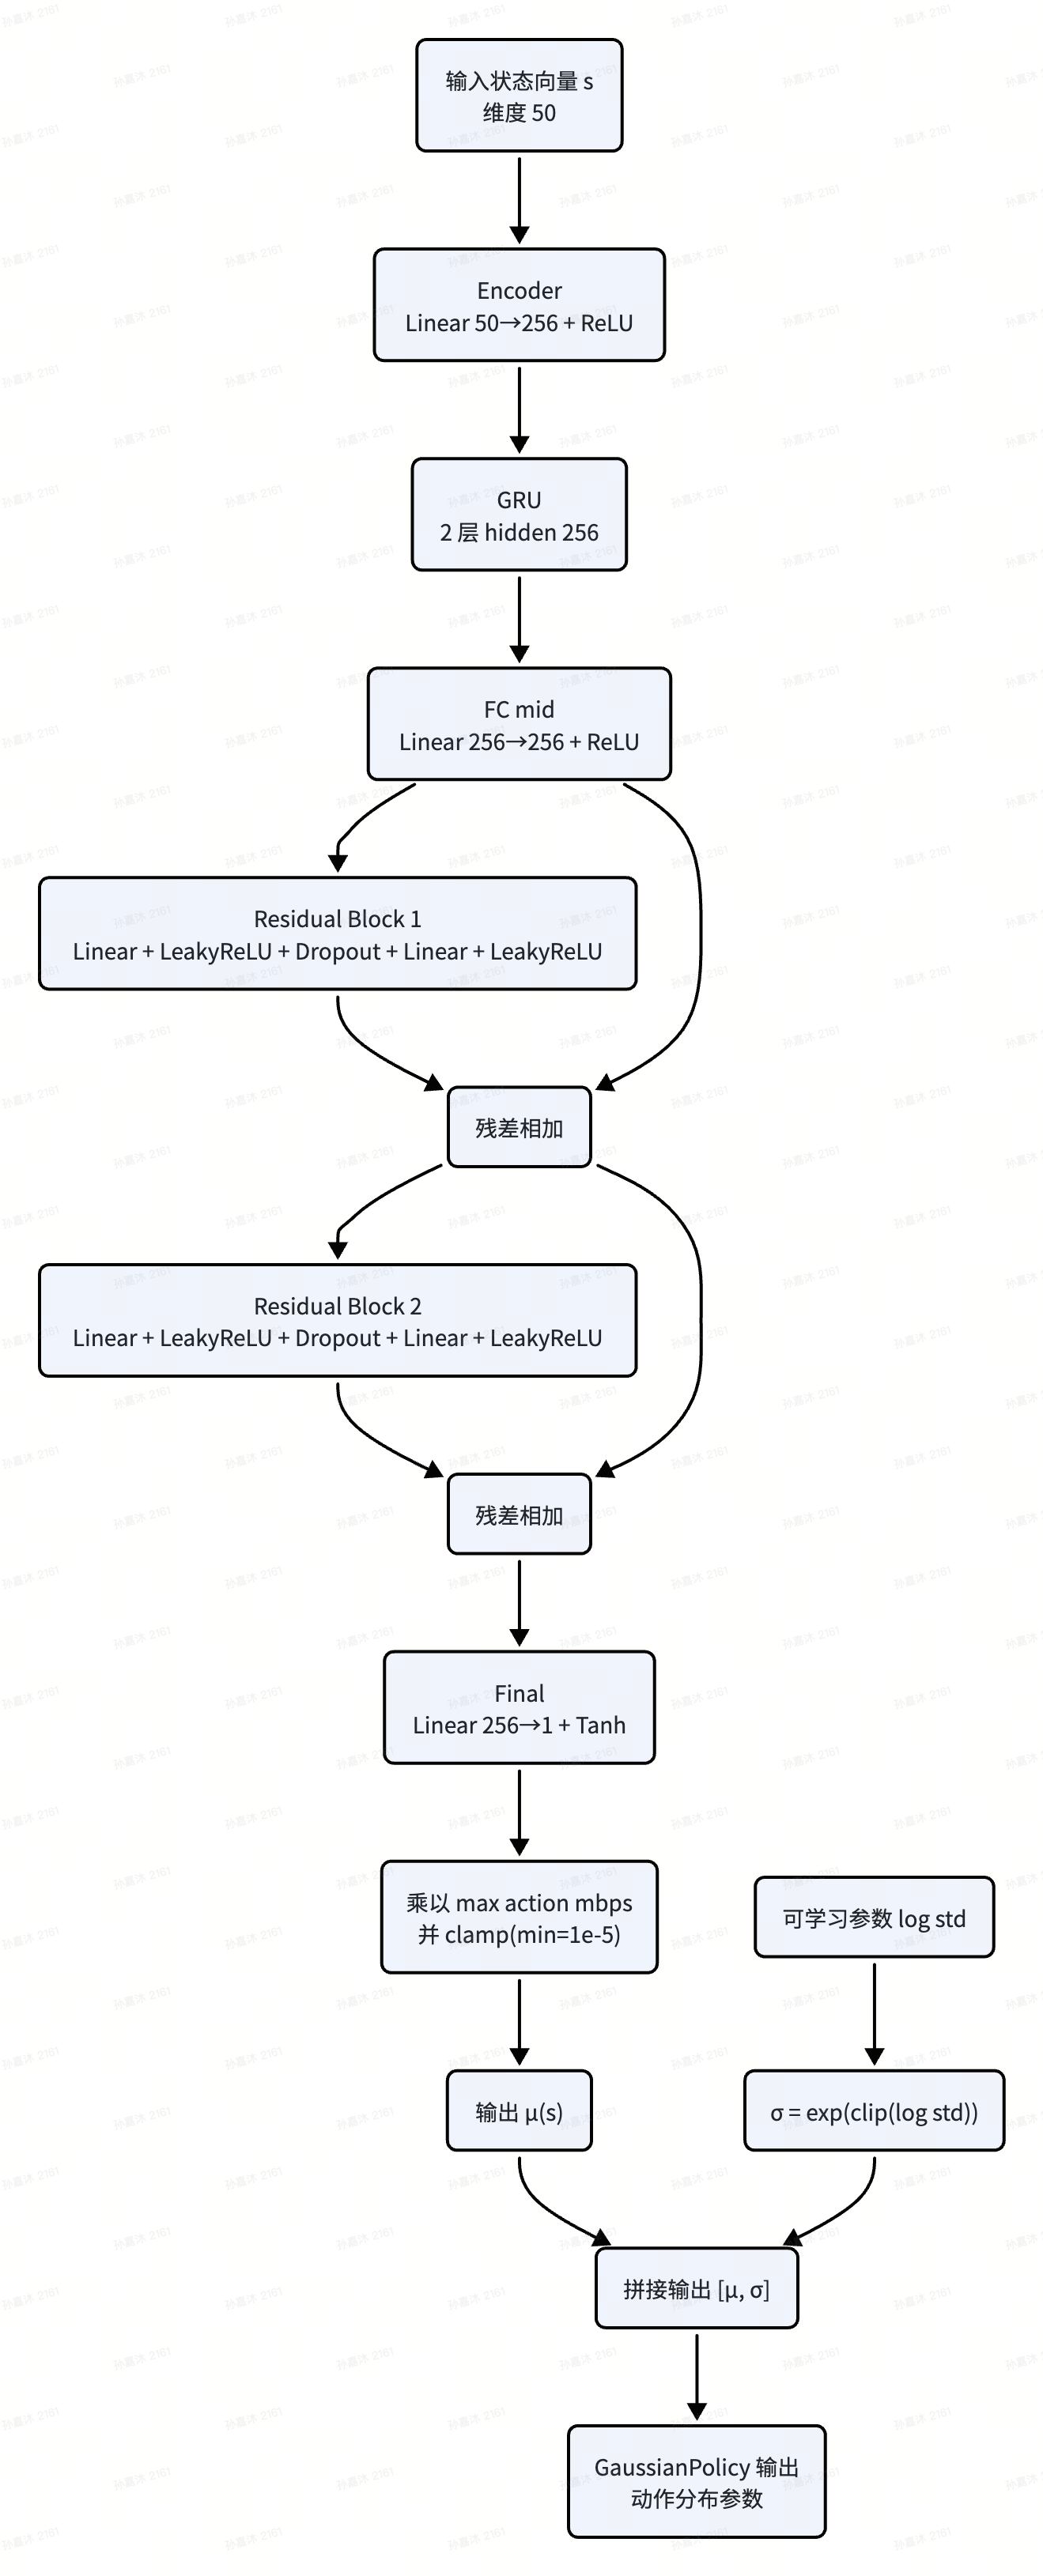
\includegraphics[width=0.5\textwidth]{figures/chapter5/5-1_GaussianPolicy.png}
    \caption{GaussianPolicy 策略网络结构示意}
    \label{fig:gaussian-policy-arch}
\end{figure}

策略网络采用高斯形式而非确定性形式，即在状态 $s$ 下输出条件分布 $\mathcal{N}(\mu(s), \sigma^2)$。其中标准差 $\sigma$ 不依赖网络前向计算，而是作为独立的可学习参数 \texttt{log\_std}（截断于 $[-20, 2]$）存在。该设计不仅参数高效，更使训练过程的不确定性表达可控、可观测——较大 $\sigma$ 反映探索阶段，收敛后的较小 $\sigma$ 则表征策略的确定性程度。在推理阶段本研究直接采用均值 $\mu(s)$ 作为输出动作，以避免随机抖动对视频编码器码率配置的扰动。

价值网络则采用更轻量的 MLP 结构（两层 256 维隐藏单元）。考虑到拥塞控制任务的输入维度较低（50 维），过深的价值网络容易过拟合数据噪声。Q 网络采用\textbf{Twin Q}架构以抑制过估计偏差：维护两个独立初始化的 Q 网络 $Q_1$、$Q_2$，目标值计算时取 $\min(Q_1, Q_2)$。在离线场景下，数据稀疏区域的 Q 值过估计将引导策略偏离行为支撑集，Twin Q 通过最小化操作显著降低了两个网络同时高估同一区域的概率。

\section{基于 IQL 的训练目标与训练流程}

IQL 算法的核心创新在于以\textbf{期望回归}（Expectile Regression）替代传统 Q 学习中的 $\max_a Q(s,a)$ 操作。后者在离线场景下会因数据集中未出现动作的 Q 值估计不可靠而引入严重过估计；前者则通过不对称 L2 损失估计 Q 值分布的高分位点，从而在不显式访问分布外动作的前提下提取策略改进信号。具体地，价值函数通过最小化
\[
\mathcal{L}_V(\theta) = \mathbb{E}_{(s,a) \sim \mathcal{D}} \left[ L_2^\tau \left( Q_{\hat{\theta}}(s,a) - V_\theta(s) \right) \right], \quad L_2^\tau(u) = |\tau - \mathbb{I}(u < 0)| \cdot u^2
\]
进行训练。当 $\tau > 0.5$ 时，损失对正残差赋予更大权重，使 $V(s)$ 收敛至 $Q$ 值分布的高分位点而非均值。本研究采用 $\tau = 0.7$，使价值函数能够自动识别数据集中的“好动作”，无需遍历所有可能动作即可估计接近最优的状态价值。

Q 函数的更新沿用标准 Bellman 方程，但目标值由价值函数 $V$ 而非 $Q$ 自身回引：
\[
y = r + \gamma (1 - d) V(s'), \quad \mathcal{L}_Q(\phi) = \mathbb{E}_{(s,a,r,s',d) \sim \mathcal{D}} \left[ \left( Q_\phi(s,a) - y \right)^2 \right].
\]
该设计避免了 Q 函数自举（bootstrap）带来的累积误差，因为 $V(s')$ 已通过期望回归从数据中提取了稳定估计。目标 Q 网络通过软更新 $\theta_{\text{target}} \leftarrow (1-\tau_s) \theta_{\text{target}} + \tau_s \theta_{\text{online}}$（$\tau_s = 0.005$）平滑追踪在线 Q 网络。

策略网络则通过\textbf{优势加权行为克隆}进行优化：
\[
\mathcal{L}_\pi(\psi) = \mathbb{E}_{(s,a) \sim \mathcal{D}} \left[ \exp(\beta \cdot A(s,a)) \cdot \left(-\log \pi_\psi(a|s)\right) \right],
\]
其中优势函数 $A(s,a) = Q(s,a) - V(s)$ 衡量动作相对于平均水平的优劣。指数权重 $\exp(\beta \cdot A)$ 使高优势动作主导梯度方向，引导策略向数据集中“更好的子集”靠拢；而对负优势动作的权重抑制则防止策略偏离数据支撑集。本研究取 $\beta = 3.0$，并将指数权重截断至 100 以避免极端样本主导训练。当 $\beta \to 0$ 时该目标退化为普通行为克隆，无法实现策略改进；过大的 $\beta$ 又会引入训练不稳定性，二者之间的权衡是 IQL 调参的关键。

\ref{fig:iql-training-overview} 概括了三类网络在单步更新中的数据流与执行顺序，完整训练超参数列于\autoref{tab:iql-hparams}。其中折扣因子 $\gamma = 0.99$ 强调拥塞控制决策的长期累积效应——当前时刻的带宽估计将在后续数秒内持续影响编码器码率与队列状态；最大动作值则取自训练数据动作分布的 99.5\% 分位点的 1.05 倍（约 12 Mbps），在覆盖大多数场景的同时避免对极端异常的过拟合。

\begin{figure}[htbp]
    \centering
    \begin{minipage}{0.40\textwidth}
        \centering
        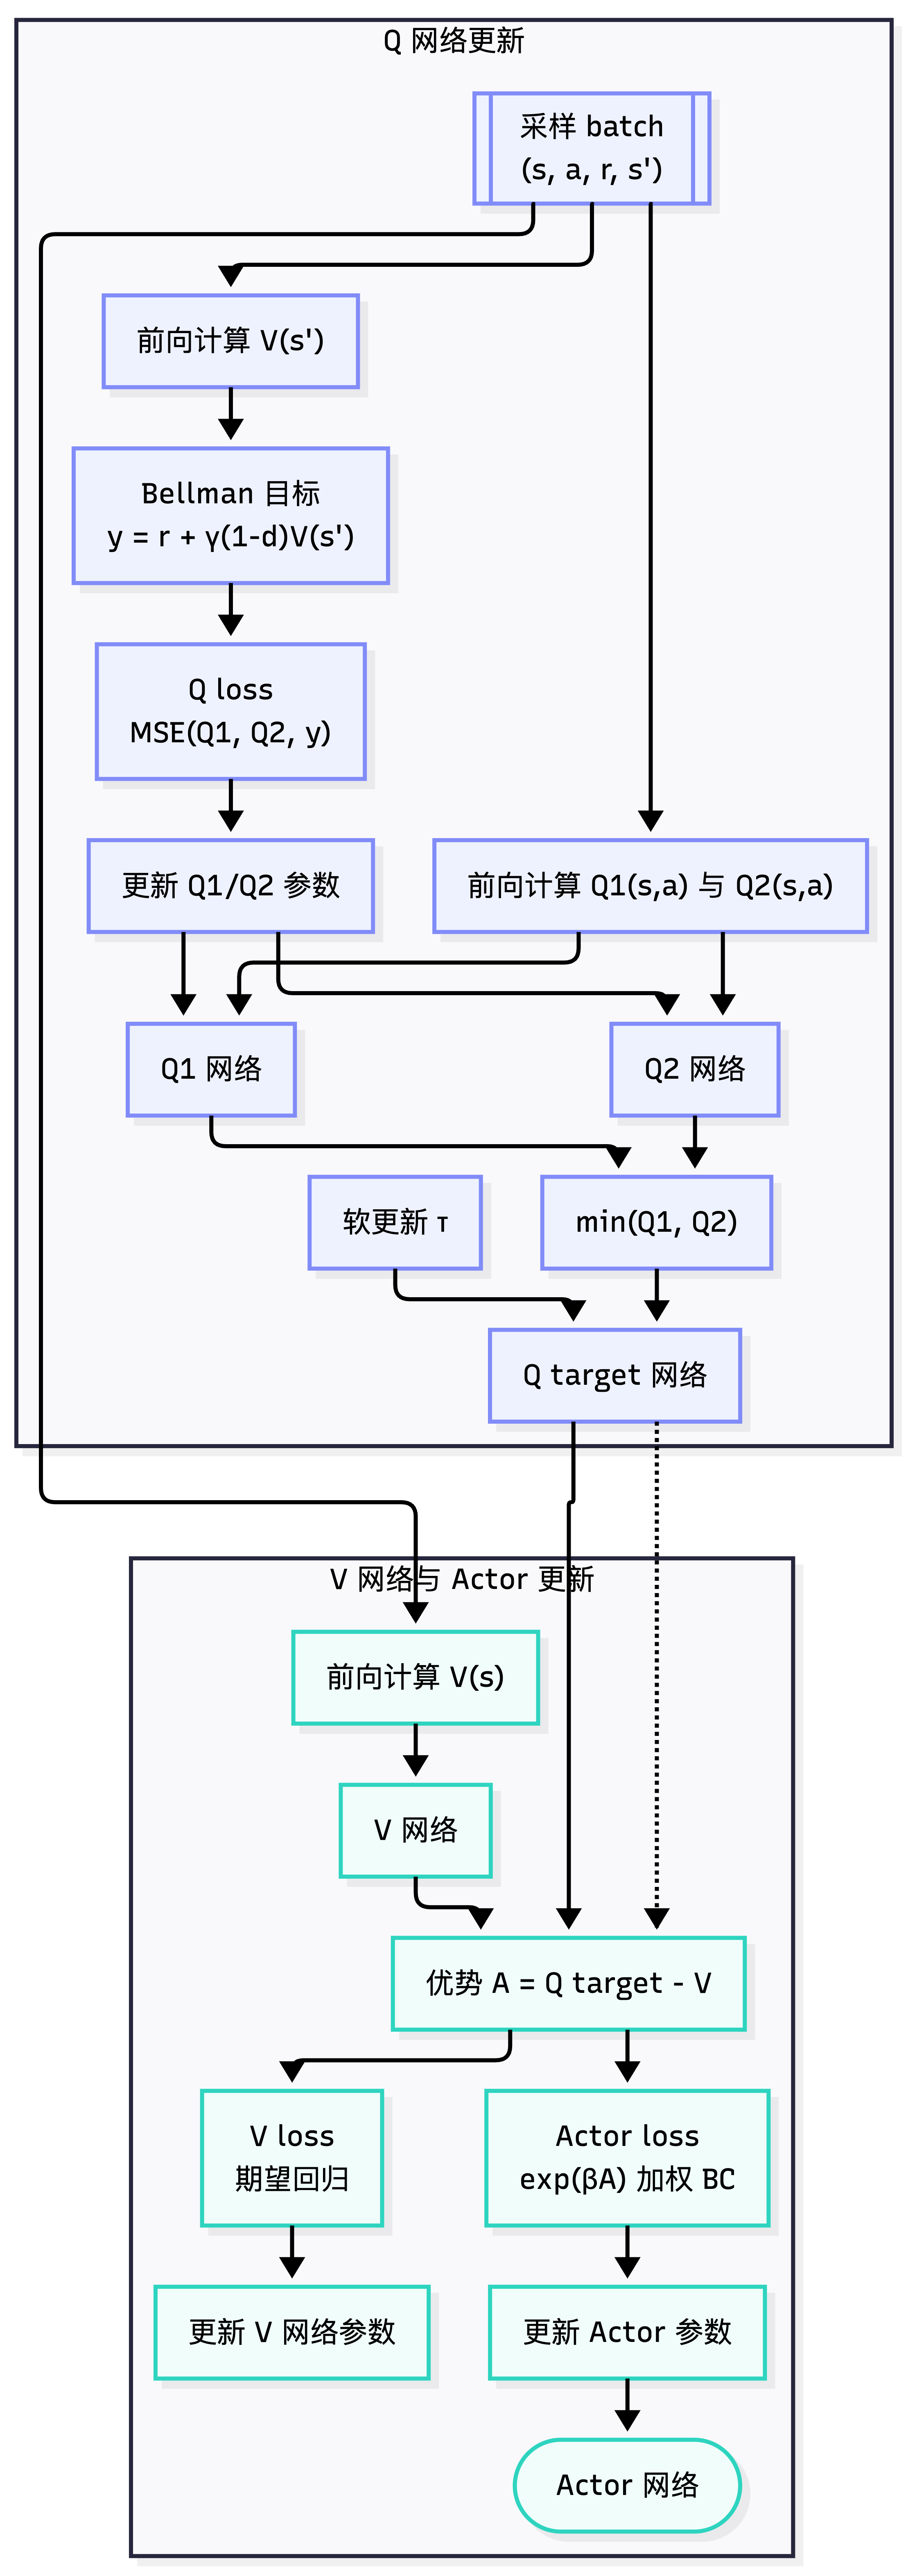
\includegraphics[width=\textwidth]{figures/chapter5/5-2_three_network.png}
    \end{minipage}\hfill
    \begin{minipage}{0.30\textwidth}
        \centering
        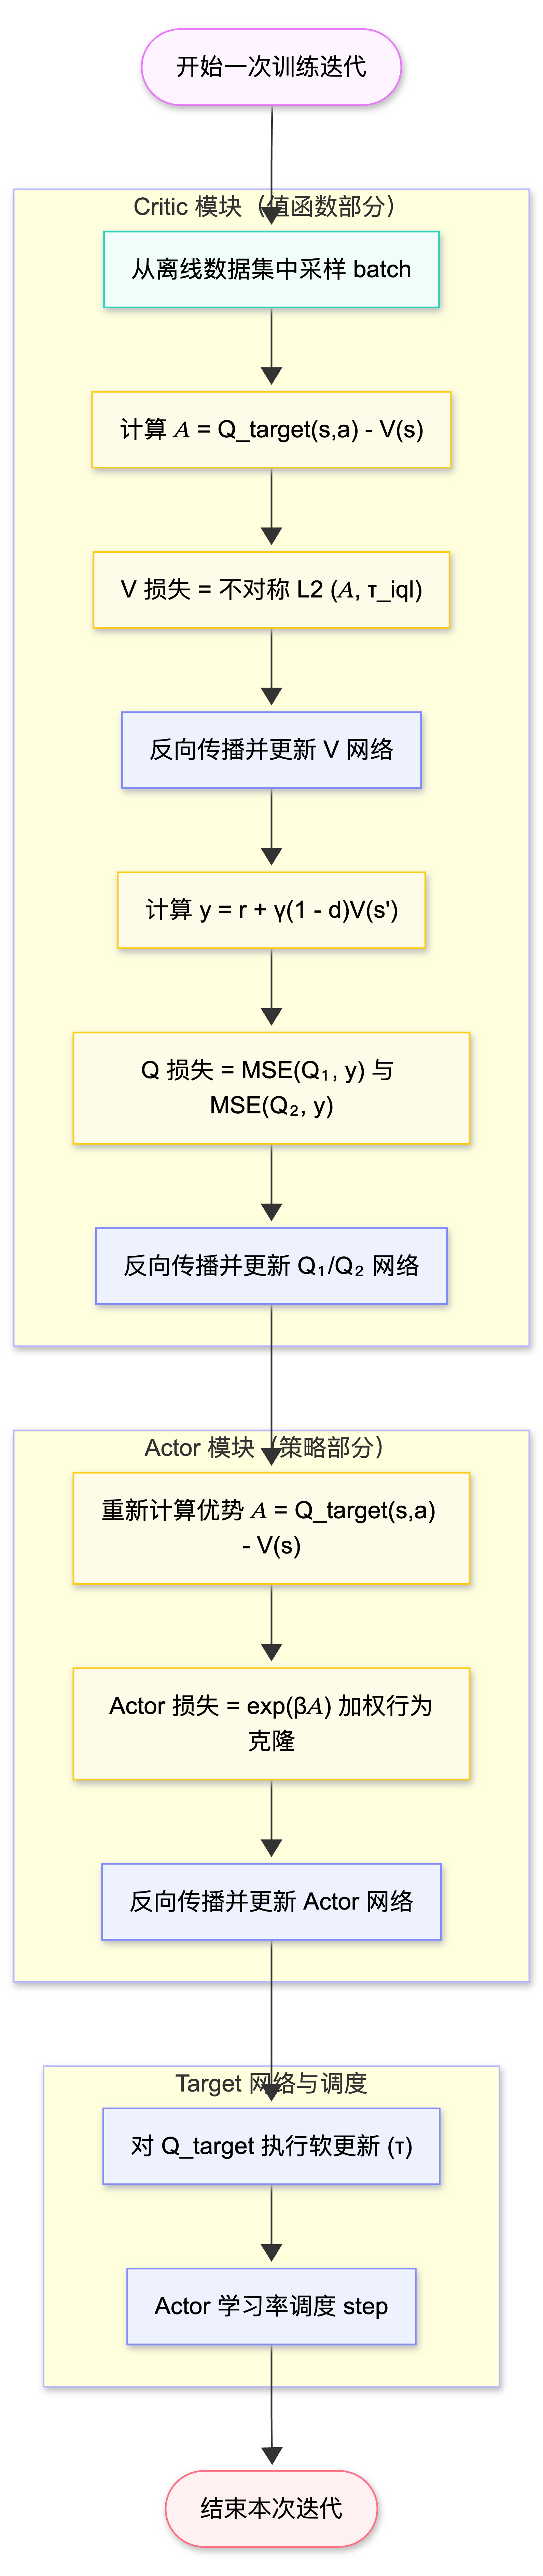
\includegraphics[width=\textwidth]{figures/chapter5/5-3_iql_false_code.png}
    \end{minipage}
    \caption{IQL 训练流程与损失构成示意}
    \label{fig:iql-training-overview}
\end{figure}

\begin{table}[htbp]
    \centering
    \begin{tabular}{|l|l|l|}
        \hline
        超参数 & 取值 & 说明 \\
        \hline
        训练步数 $T$ & 300{,}000 & 总优化迭代次数 \\
        批量大小 $B$ & 512 & 每步采样数 \\
        折扣因子 $\gamma$ & 0.99 & 长期奖励折扣 \\
        软更新系数 $\tau_s$ & 0.005 & Target Q 跟踪速率 \\
        期望回归参数 $\tau_{\text{IQL}}$ & 0.7 & 价值函数分位数 \\
        逆温度系数 $\beta$ & 3.0 & 优势加权强度 \\
        学习率 $\eta$ & $3 \times 10^{-4}$ & 全网络统一 \\
        梯度裁剪阈值 & 1.0 & 数值稳定保护 \\
        最大动作值 & $\sim 12$ Mbps & 动作空间上界 \\
        \hline
    \end{tabular}
    \caption{IQL 训练超参数配置}
    \label{tab:iql-hparams}
\end{table}

训练循环以标准方式从 ReplayBuffer 中采样并依次执行价值更新、Q 函数更新、策略更新与目标网络软更新，每 5000 步在预留验证集（占 10\%）上评估一次并保存中间状态。验证阶段以\textbf{负对数似然}（NLL）作为主要监控指标，原因在于高斯策略的优化目标本质上是最大化数据动作在策略分布下的似然，NLL 同时惩罚均值偏差与不合理的方差估计，能够区分“均值拟合差”与“通过增大方差掩盖误差”两种失效模式，比单纯的 MSE 更贴合训练目标。\ref{fig:training-loss-curves} 与\ref{fig:actor-learning-curve} 展示了训练过程中关键损失与 Actor 学习曲线的演化趋势，可见各损失均稳定下降且未出现 Q 值崩溃或 NLL 反弹的异常现象。需指出，离线验证指标仅反映策略对行为策略的拟合程度，并不直接代表真实环境中的控制性能，后者需通过\ref{chap:ab-test} 章的在线 A/B 测试加以验证。

\begin{figure}[htbp]
    \centering
    \begin{minipage}{0.49\textwidth}
        \centering
        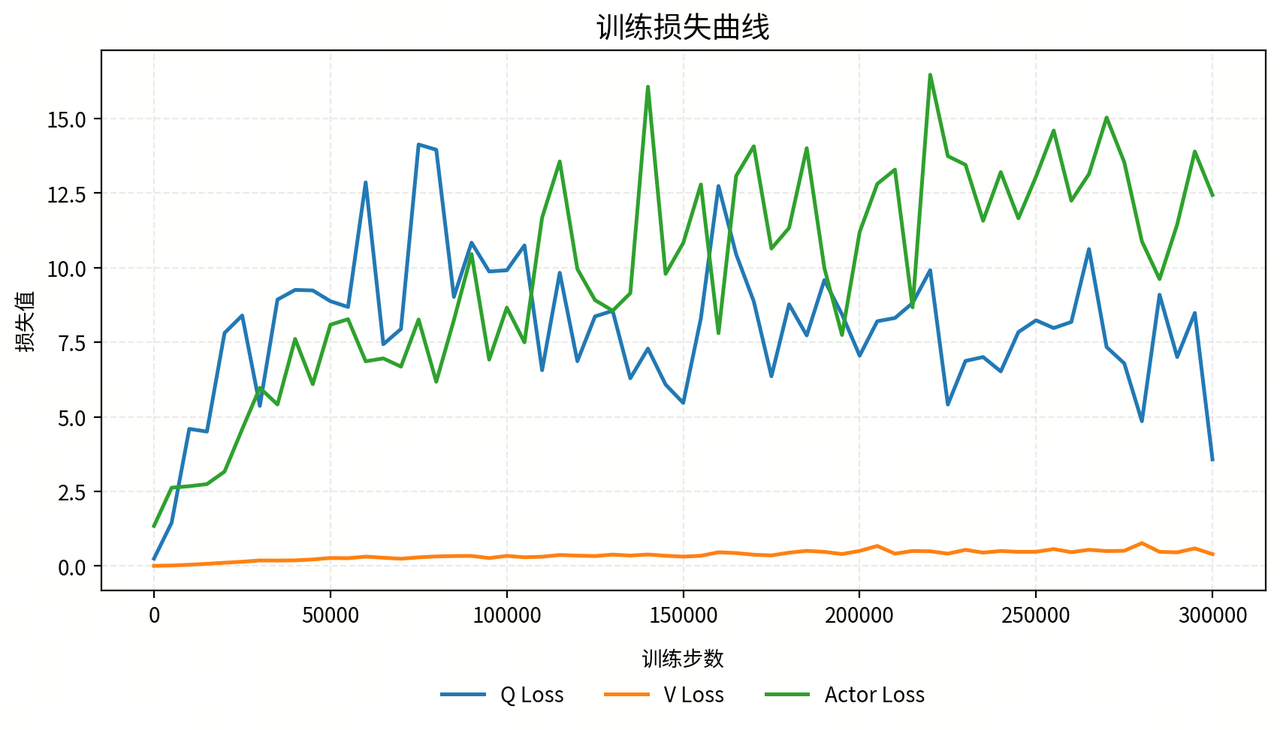
\includegraphics[width=\textwidth]{figures/chapter5/5-4_loss_curse.png}
    \end{minipage}\hfill
    \begin{minipage}{0.49\textwidth}
        \centering
        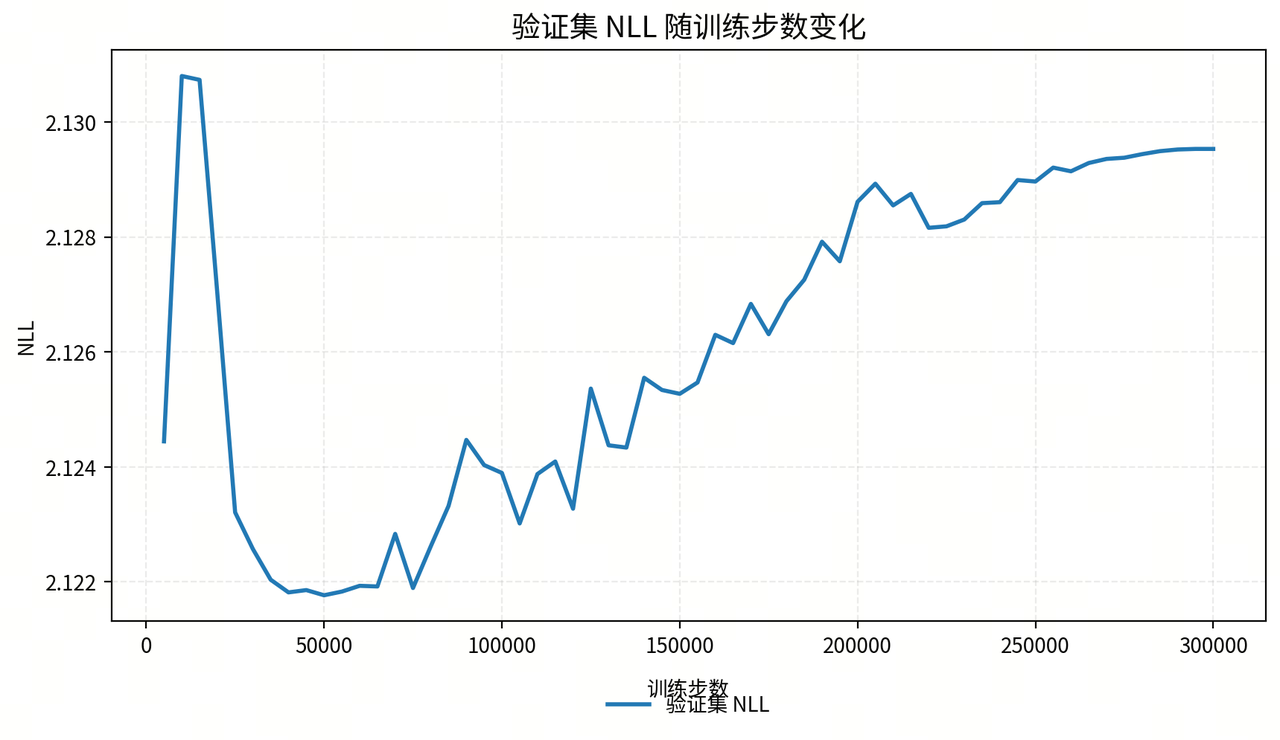
\includegraphics[width=\textwidth]{figures/chapter5/5-5_NLL curve.png}
    \end{minipage}
    \caption{训练过程关键损失曲线}
    \label{fig:training-loss-curves}
\end{figure}

\begin{figure}[htbp]
    \centering
    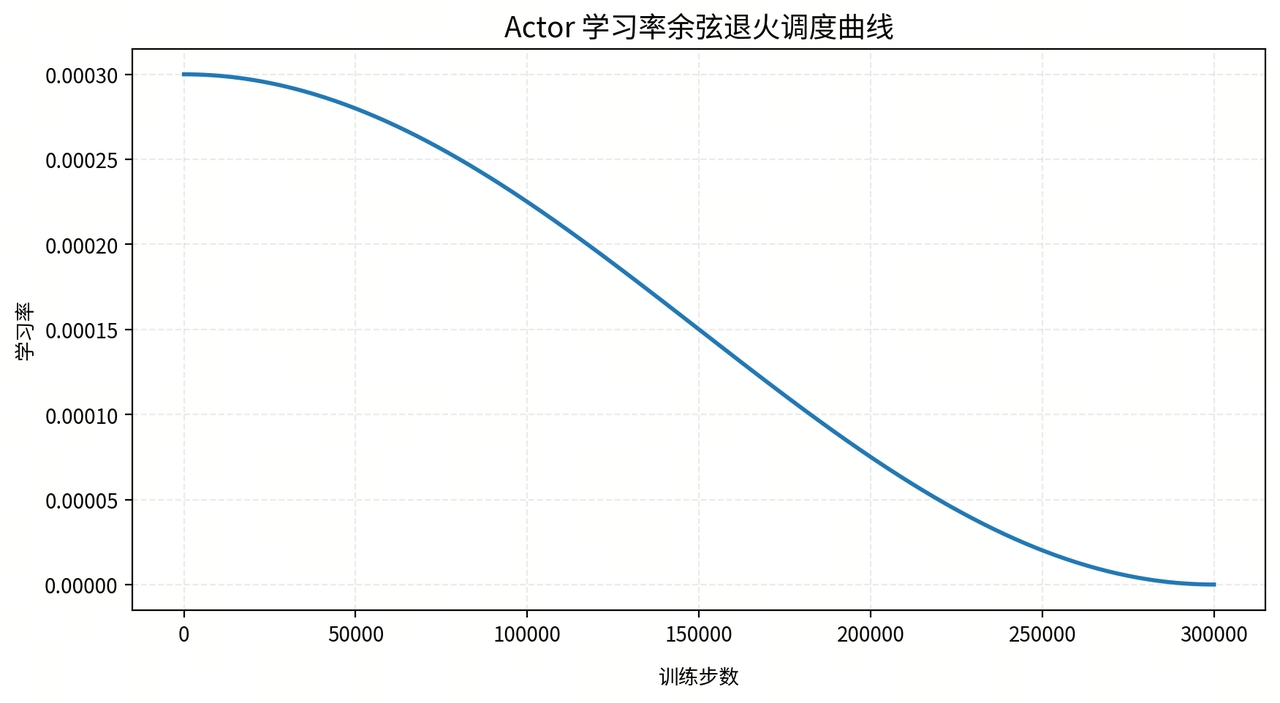
\includegraphics[width=0.75\textwidth]{figures/chapter5/5-6_Actor_learning_curve.png}
    \caption{Actor 学习曲线}
    \label{fig:actor-learning-curve}
\end{figure}

训练完成后，本研究以 checkpoint 形式持久化策略网络、Twin Q 网络、训练状态与归一化元信息，并固定随机种子以保证实验可复现。

\section{模型部署架构的演进与一致性保证}

训练好的策略需要嵌入实际的 WebRTC 控制回路才能产生效益，而部署形态的选择直接决定了推理的实时性和有效性。本研究在初期阶段采用了方案 A：远端 Python HTTP/WebSocket 推理服务——将 PyTorch 模型部署在服务端，前端通过 HTTP/WebSocket 上报状态向量并接收带宽估计。该方案与训练运行时完全一致，调试工具链完整，能够快速验证“采集—训练—部署”全链路的逻辑正确性，并支持不重新部署前端的情况下进行模型热更新。

然而，将方案 A 投入差网络场景的 A/B 测试时，一个根本性的工程矛盾浮现：越是劣化的网络条件下，RL 实验组的表现反而越不稳定。深入分析后发现，问题的根源不在模型本身，而在于推理请求所依赖的 TCP/WebSocket 链路与被测试的 WebRTC 媒体链路共享同一条物理信道。当信道进入拥塞状态时，推理请求自身遭遇排队延迟乃至丢包重传，导致策略决策在最需要快速响应的时刻反而出现数十毫秒至上百毫秒的滞后。这一滞后使模型基于“过时”的网络状态产生输出，与 RTCP 反馈的实际状态发生相位错位，从而在网络恢复时做出错误的保守决策、在网络恶化时反应不及——形成“控制滞后→拥塞加剧→推理更慢”的恶性循环。

这一发现驱动本研究转向\textbf{方案 B：浏览器本地 ONNX 边缘推理}。将训练得到的策略网络以 opset 17 导出为 ONNX 计算图（流程见图\ref{fig:onnx-export}）。在导出后使用 ONNX Runtime 对策略网络重新加载，在相同输入下与 PyTorch 原始模型逐元素对比输出张量，要求最大绝对偏差不超过 $10^{-5}$ ，从而确认 ONNX 计算图忠实复现了原模型的数值行为。前端基于 \texttt{onnxruntime-web} 在浏览器进程内完成推理，并重建了与训练侧语义对齐的因果特征清洗与状态归一化流水线，从而将完整的控制回路封闭在客户端进程中（控制回路结构见图\ref{fig:policy-runtime}）。迁移之后，推理延迟从差网络下的数十至上百毫秒骤降至亚毫秒级，且与底层信道状态完全解耦，A/B 测试评估结果随之变得稳定可解释。

\begin{figure}[htbp]
    \centering
    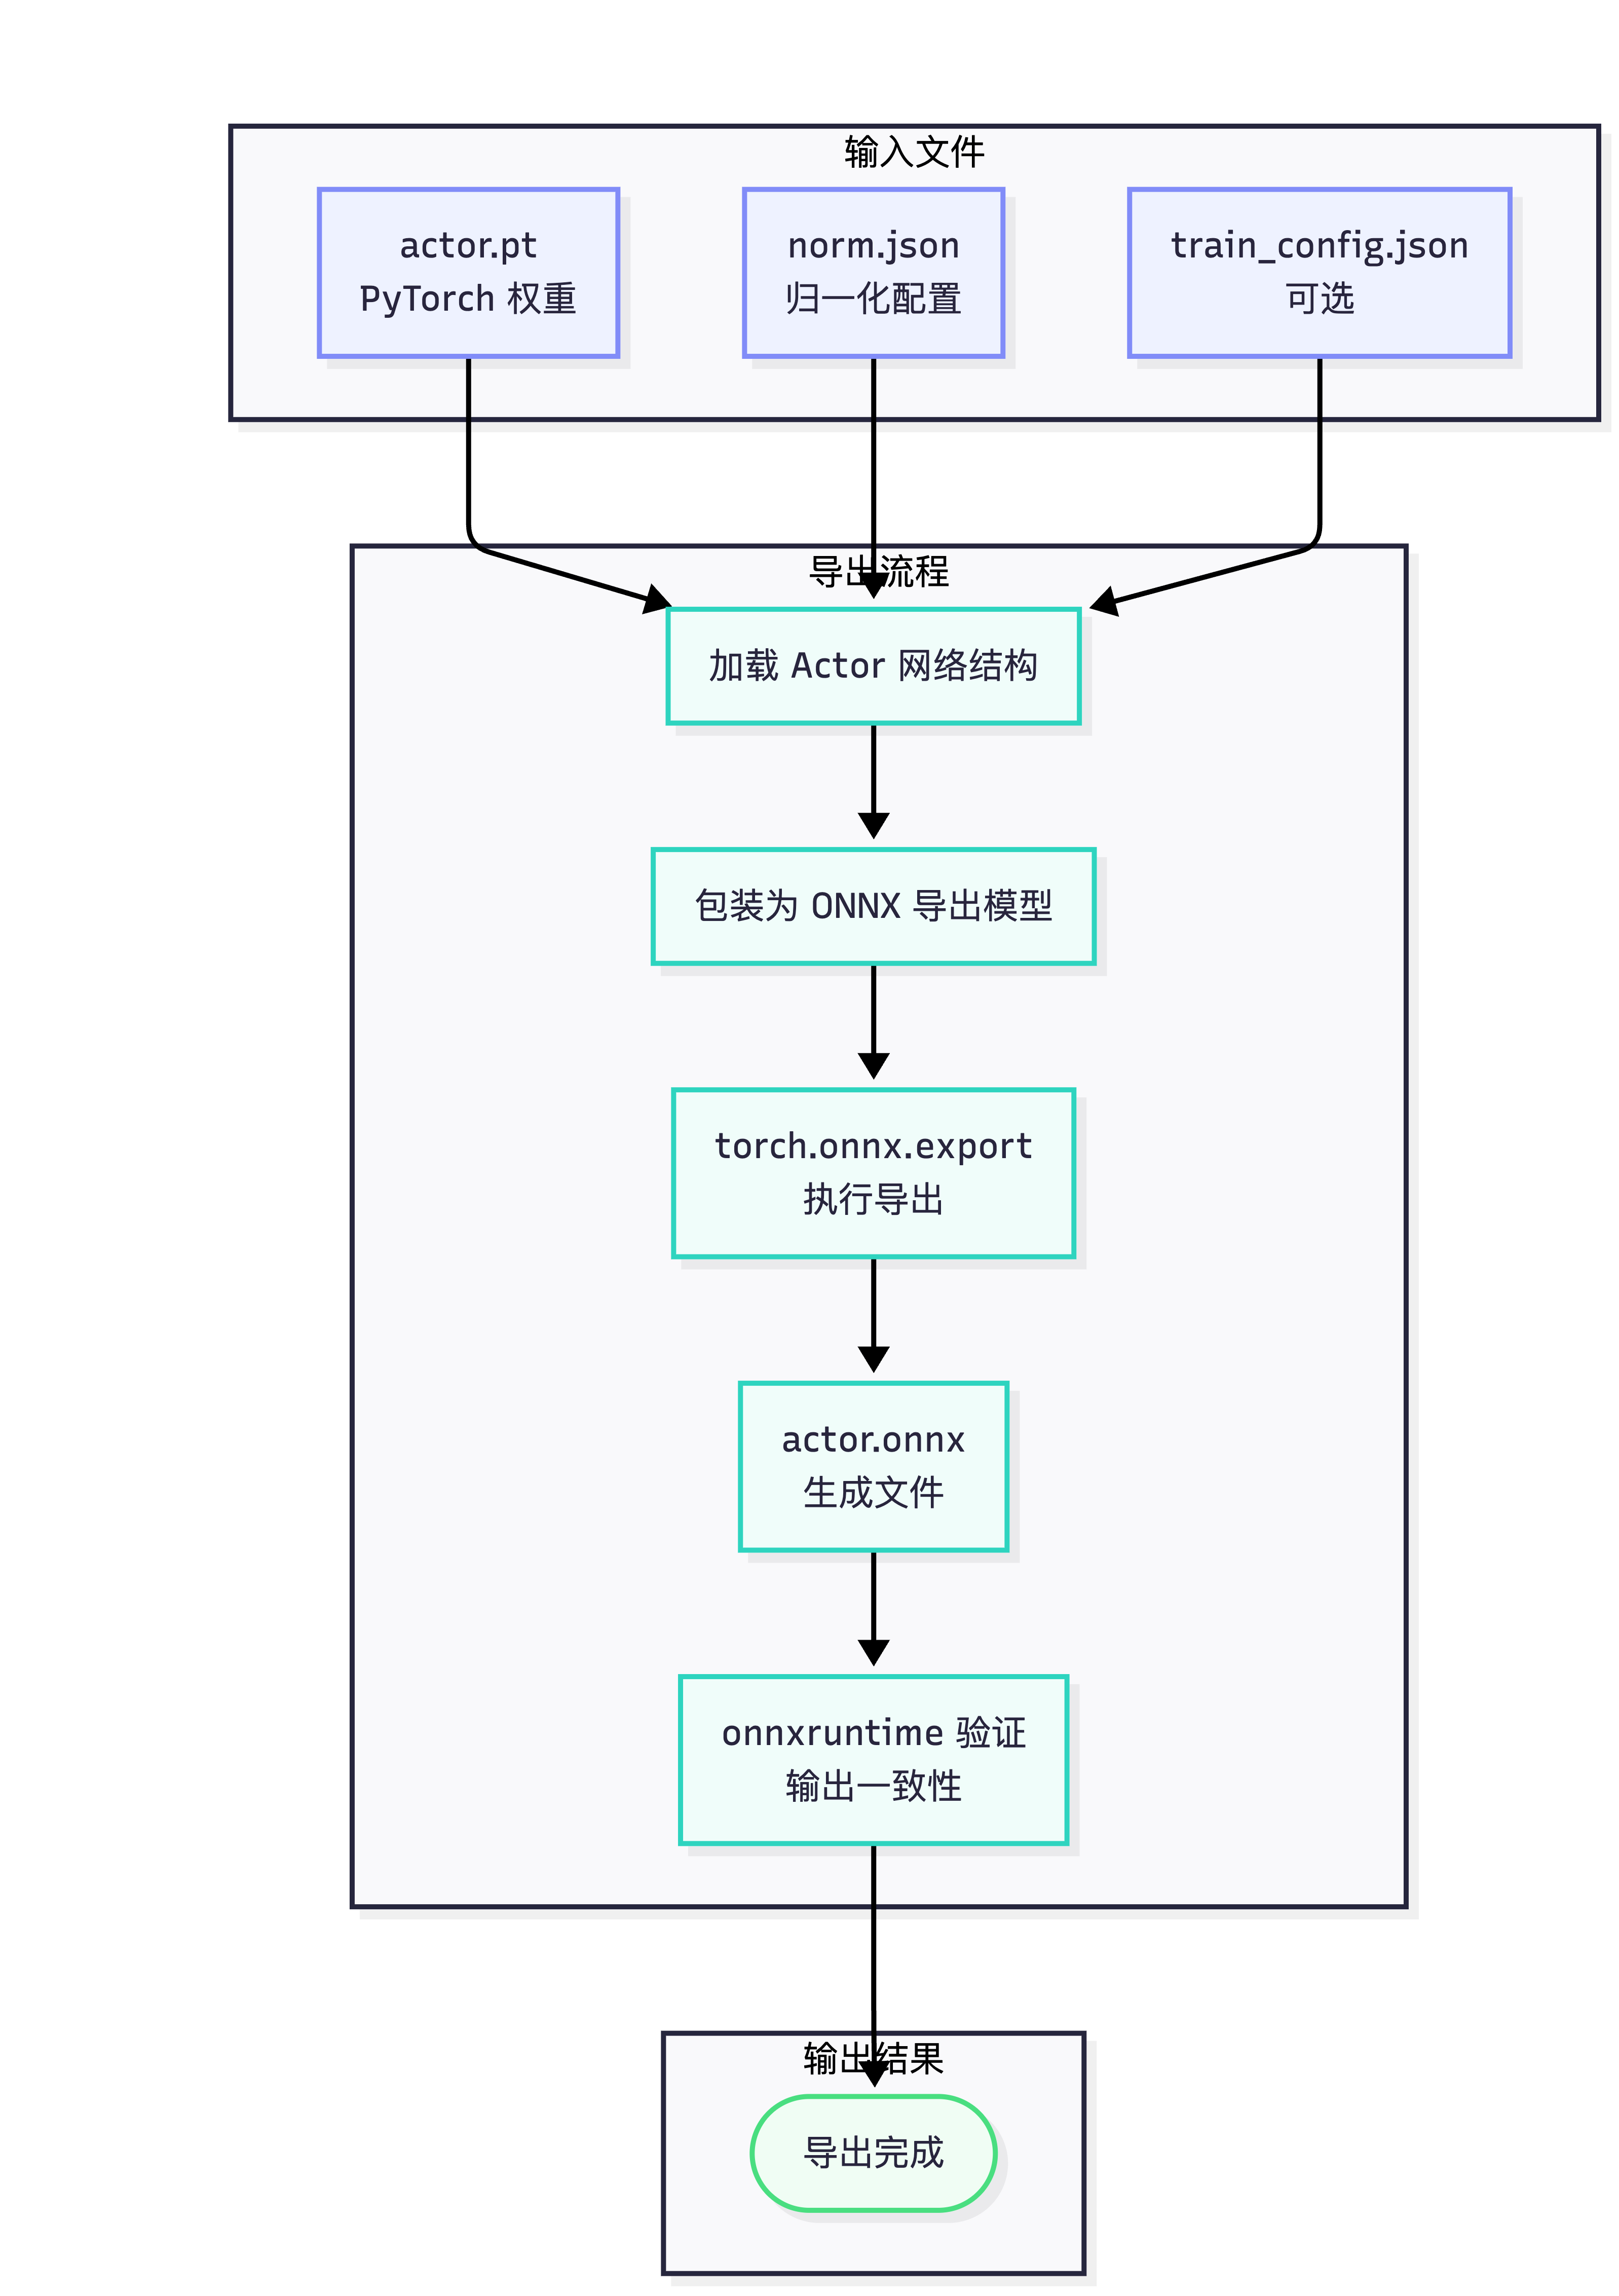
\includegraphics[width=0.9\textwidth]{figures/chapter5/5-7_onnx_output.png}
    \caption{ONNX 模型导出与一致性校验流程}
    \label{fig:onnx-export}
\end{figure}

\begin{figure}[htbp]
    \centering
    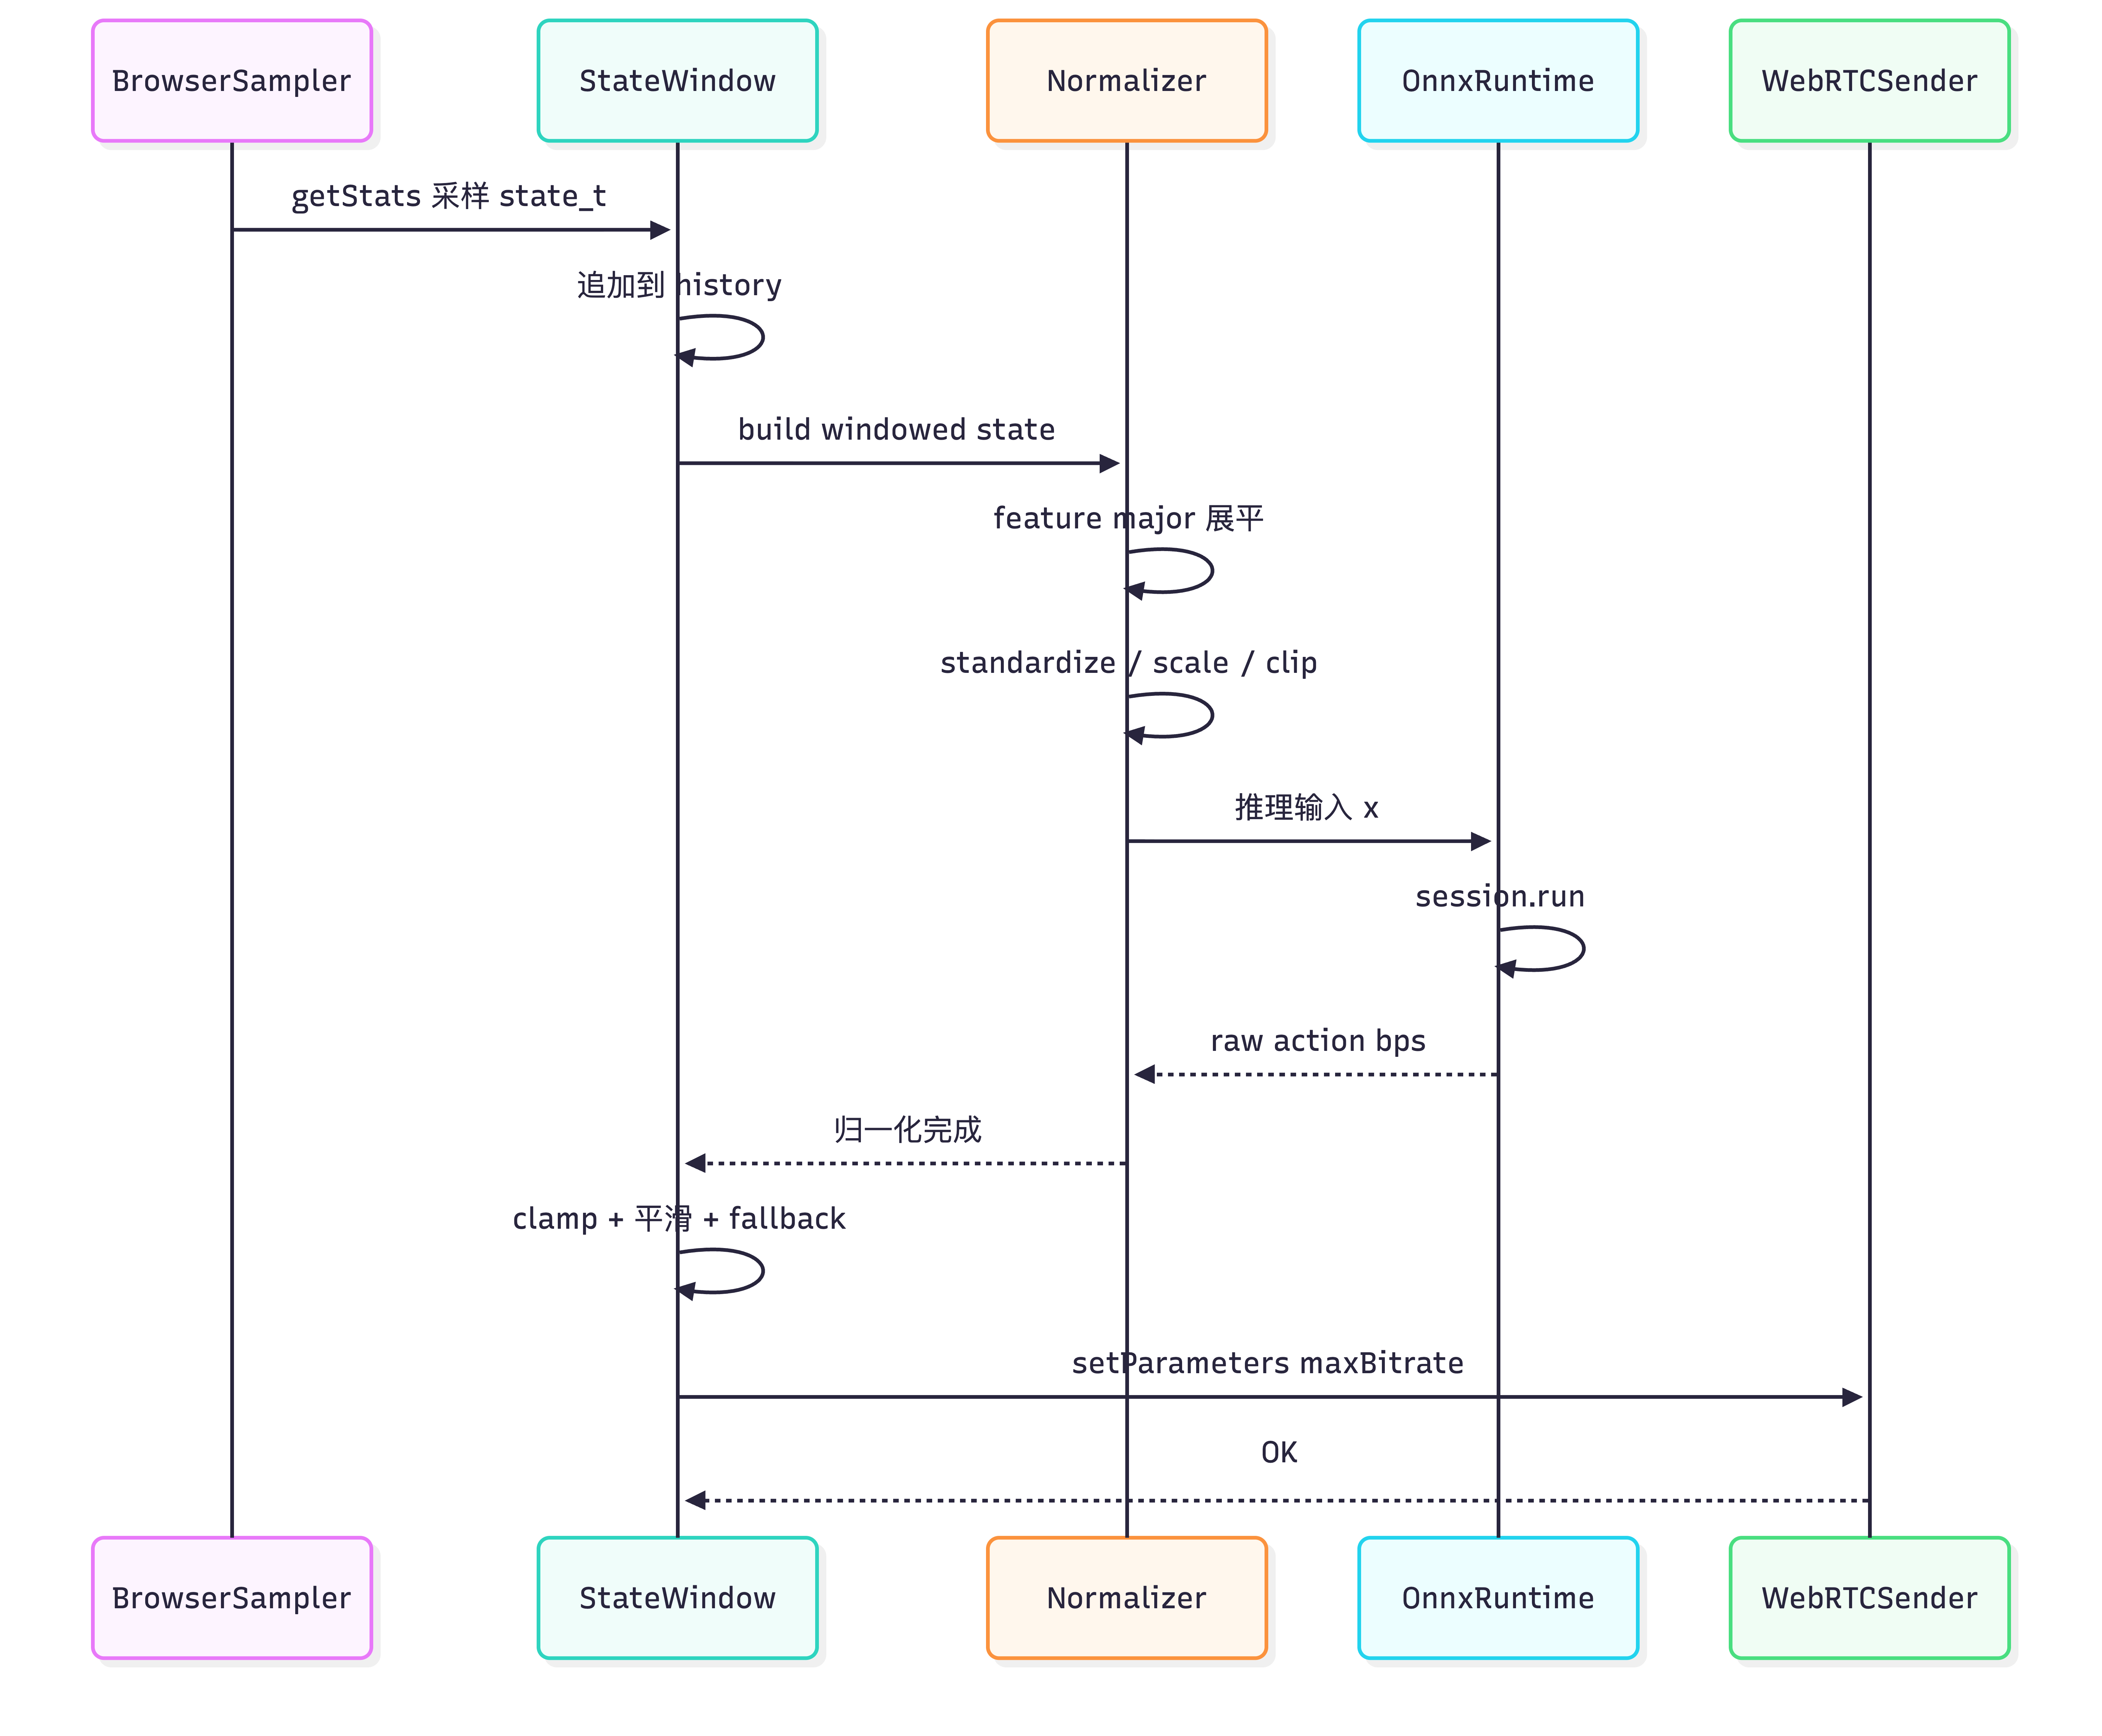
\includegraphics[width=0.9\textwidth]{figures/chapter5/5-8_policy_runtime.png}
    \caption{浏览器端 ONNX 推理与控制回路结构}
    \label{fig:policy-runtime}
\end{figure}

最终本研究保留了“方案 A 作为算法调试与单机验证的辅助通道、方案 B 作为真实 A/B 测试的主干部署形态”的双栈架构。两种方案分别回答“模型逻辑是否符合预期”与“策略在真实 RTC 系统中能否带来 QoE 提升”两个不同维度的问题，二者的性能与适用场景对比见表\ref{tab:deployment-forms}。这一技术演进过程亦提示了一条普适经验：在实时控制系统中引入深度学习策略时，推理链路与被控系统的耦合关系必须作为架构设计的首要约束，不能等同于传统离线服务的部署思路。

\begin{table}[htbp]
    \centering
    \begin{tabular}{|l|l|l|}
        \hline
        维度 & HTTP/WebSocket 服务 & ONNX 浏览器本地 \\
        \hline
        推理延迟（LAN） & 5–20 ms & $<$1 ms \\
        推理延迟（差网络） & 50–300 ms & $<$1 ms \\
        与媒体流耦合 & 强耦合（共享信道） & 完全解耦 \\
        调试能力 & 完整 & 受限 \\
        部署依赖 & 需后端服务 & 仅需静态文件 \\
        \hline
    \end{tabular}
    \caption{两种推理部署形态对比}
    \label{tab:deployment-forms}
\end{table}

无论选择哪一形态，训练-部署一致性都是策略能否被忠实复现的前提。本研究通过三方面机制保障一致性：其一，状态归一化的尺度系数与截断范围同时存储于训练侧的 \texttt{norm.json} 与前端部署脚本中，确保两端的数值处理完全相同；其二，动作空间在训练与部署阶段均以 Mbps 为内部单位、仅在边界处与 bps 相互转换，避免单位混淆；其三，ONNX 导出后强制执行 PyTorch-ONNX 的输出对齐校验。

\section{本章小结}

本章完整描述了基于 IQL 的拥塞控制模型从离线训练到在线部署的技术路径。在范式选择上，本章论证了离线强化学习相较于在线学习在 WebRTC 场景下的必要性，并阐释了 IQL 通过期望回归规避分布外动作评估的核心思想。在网络架构设计上，本章构建了线性编码—双层 GRU—残差块—Tanh 输出的高斯策略网络，并配以 Twin Q 与独立价值网络以抑制过估计。在训练流程上，本章通过期望回归（$\tau_{\text{IQL}}=0.7$）训练价值函数，以优势加权行为克隆（$\beta=3.0$）更新策略，并采用软目标更新与梯度裁剪保证数值稳定性，最终选取 NLL 作为主要离线验证指标以契合高斯策略的优化目标。在部署架构上，本章呈现了从“远端 Python 推理”到“浏览器端 ONNX 边缘推理”的工程演进，揭示了实时控制系统中推理链路与被控系统耦合关系的核心约束，并通过三类机制保证训练-部署一致性。上述工作使离线强化学习策略具备了在真实 WebRTC 通信链路中替代或增强 GCC 进行码率控制的工程能力，为下一章的在线 A/B 测试评估奠定了基础。
